% !TEX root =  ../main_manuscript.tex 
\section{Simulation Study}
\label{sec:sim_study}
Although we demonstrated personalized schedules for a real patient, we also intend to analyze and compare personalized and fixed schedules in a full study cohort. We use two measures for this comparison, namely, the number of invasive tests in a schedule, and the actual time delay in detection of progression for each schedule. To this end, the ideal option of a randomized clinical trial of test schedules is infeasible. In addition, due to the periodical nature of schedules the actual time delay in detection of progression in real world surveillance is unobservable. Hence, we instead conduct an extensive simulation study to compare personalized versus fixed schedules. To keep our simulation study realistic, we employ the prostate cancer active surveillance scenario. More specifically, we utilize the joint model fitted to the PRIAS cohort to generate simulated cohorts that are replicas of PRIAS.

\subsection{Simulation Setup}
From the simulation population, we first sample 500 datasets, each representing a hypothetical prostate cancer active surveillance program with 1000 patients in it. We generate a true cancer progression time for each of the ${\mbox{500} \times \mbox{1000}}$ patients and then sample a set of longitudinal DRE and PSA measurements at the same follow-up visit times as given in the PRIAS protocol. We then split each dataset into training (750 patients) and test (250 patients) parts, and generate a random and non‐informative censoring time for the training patients. All test and training patients also observe Type-I censoring at year ten of follow-up (current study period of PRIAS). We next fit a joint model of the same specification as the model fitted to PRIAS (Web-Appendix~B), to each of the 500 training datasets and obtain MCMC samples from the 500 sets of the posterior distribution of the parameters. In each of the 500 hypothetical surveillance programs, we utilize the corresponding fitted joint models to develop the profiles for cumulative-risk of progression in each of the ${\mbox{500} \times \mbox{250}}$ test patients. This cumulative-risk is further used to create personalized biopsy schedules for the test patients. For each test patient we conduct biopsies using the following personalized biopsy schedules: fixed risk thresholds $\kappa=5\%$, $\kappa=10\%$, and automatically chosen $\kappa_a$ (Equation~\ref{eq:kappa_choice}), and currently practiced PRIAS and annual biopsy schedules. We plan biopsies only on the standard PSA follow-up visits (Section~\ref{sec:results}) utilizing accumulated clinical data until that visit. Also, we maintain a minimum recommended gap of one year between consecutive prostate biopsies~\citep{bokhorst2015compliance}. Biopsies are conducted until progression is detected, or the maximum follow-up period at year ten (horizon) is reached. A compulsory biopsy is conducted at year ten for a fair comparison between the delays incurred in each schedule.

%This biopsy promises early detection of progression for patients misdiagnosed as low-grade cancer patients or patients who chose surveillance despite having a higher grade at diagnosis. We also . Consequently, we schedule personalized biopsies starting from year two. The added benefit of this approach is that due to the clinical data accumulated over two years, we can make reasonably accurate predictions of the cumulative-risk of progression.
\subsection{Results}
Since the simulated cohorts are based on PRIAS, roughly only 50\% of the patients progress in the ten year study period. While, we are able to calculate total number of biopsies scheduled in all $500 \times 250$ test patients, but the time delay in detection of progression is available only for those patients who progress in ten years (\textit{progressing}). We show the simulation results separately for \textit{progressing} and \textit{non-progressing} patients in Panel~A, and Panel~B of Figure~\ref{fig:simulation_boxplot}, respectively.

For \textit{progressing} patients (Panel~A,~Figure~\ref{simulation_boxplot}), we note that .....

The patients who are at the most advantage with the personalized schedules are the \textit{non-progressing} patients (Panel~B,~Figure~\ref{simulation_boxplot}). For all of these patients, annual schedule leads to 10 (unnecessary) biopsies. The schedule of the PRIAS program schedules a median of six biopsies (IQR:~4--8). In comparison,....

%Overall, we observed that the personalized schedule which uses a 10\% risk threshold at all follow-up visits is dominant over the PRIAS schedule, biennial schedule of biopsies, and biopsies every one and a half years (see~Appendix~C for the latter two schedules). This personalized schedule not only schedules fewer biopsies than the aforementioned currently practiced schedules, but the delay in detection of cancer progression is also either equal or less. The personalized schedule which uses risk threshold chosen on the basis of classification accuracy ($\mbox{F}_1$ score) is dominant over the triennial schedule (see~Appendix~C) of biopsies. The personalized schedule which uses a 5\% risk threshold schedules fewer biopsies than the annual schedule, while the delay is only trivially more than the annual schedule.

\begin{figure}
\centerline{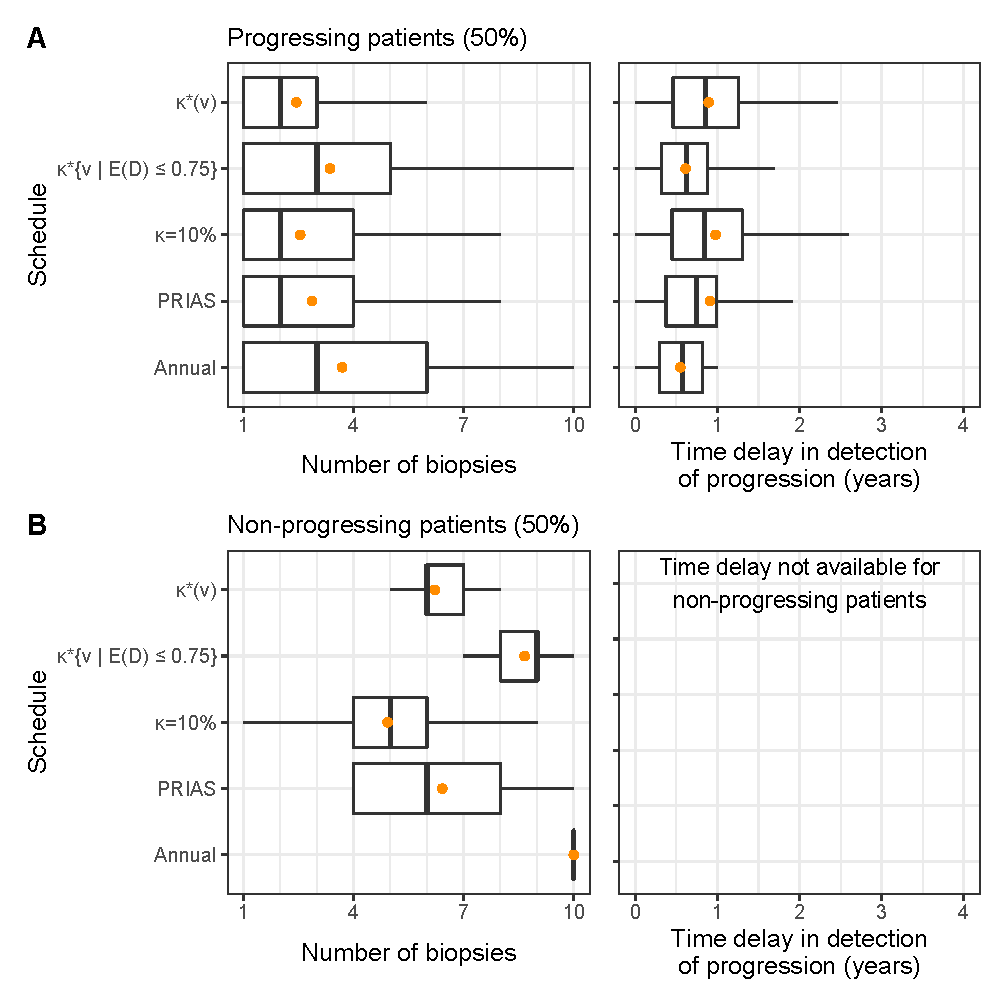
\includegraphics{images/simulation_boxplot.eps}}
\caption{\textbf{Boxplot showing variation in the number of biopsies, and the time delay in detection of cancer progression} for various biopsy schedules. Time delay (years) is calculated as (time of positive biopsy - true time of cancer progression). Biopsies are conducted until cancer progression is detected. \textbf{Panel~A:} results for simulated patients who obtained cancer progression in the ten year study period (\textit{progressing}). \textbf{Panel~B:} results for simulated patients who did not obtain cancer progression in the ten year study period (\textit{non-progressing}). Types of personalized schedules: Risk:~10\% and Risk:~5\% approaches, schedule a biopsy if the cumulative-risk of cancer progression at a visit is more than 10\% and 5\%, respectively. Risk:~Auto works similar as previous, except that a visit-specific risk threshold is chosen using Equation~(\ref{eq:kappa_choice}). Annual corresponds to a schedule of yearly biopsies and PRIAS corresponds to biopsies as per PRIAS protocol (Section~\ref{sec:results}).}
\label{fig:simulation_boxplot}
\end{figure}